\documentclass[a4paper,12pt]{article}
\usepackage{graphicx} % Required for inserting images
\usepackage{listings} % Required for inserting code snippets
\usepackage{xcolor} % Required for code highlighting
\usepackage{fancyhdr} % For better headers and footers
\usepackage{caption} % Improved captions
\usepackage{framed} % For boxed content
\usepackage{float} % For retaining image order

\title{Chat-VoIP}
\author{Ioannis Michalainas, Maria Charisi}
\date{November 2024}

% Custom settings for listings
\lstset{
    backgroundcolor=\color{gray!10}, % Light gray background for the code
    basicstyle=\ttfamily\small, % Use monospaced font, smaller size for compactness
    keywordstyle=\bfseries\color{blue!80!black}, % Distinct keyword style
    commentstyle=\color{green!50!black}, % Dimmed green comments
    stringstyle=\color{orange!80!black}, % Strings in a warm orange color
    frame=single, % Boxed with a single line
    framerule=1pt, % Thicker border for better contrast
    rulecolor=\color{black!70}, % Dark gray border color
    tabsize=4, % Standard tab size
    breaklines=true, % Automatically wrap long lines
    numbers=left, % Line numbers on the left
    numberstyle=\tiny\color{gray}, % Small and dim line numbers
    xleftmargin=15pt, % Left margin
    xrightmargin=15pt, % Right margin
    captionpos=b, % Caption below the listing
    showspaces=false, % Do not visually indicate spaces
    showstringspaces=false, % Do not visually indicate spaces in strings
    title=\colorbox{gray!20}{\ttfamily \scriptsize Code Snippet}, % Simulate an IDE title bar
    shadowbox=true, % Add a subtle shadow
    shadowsize=3pt, % Size of shadow
    shadowrule=0.4pt, % Width of shadow line
    shadowcolor=\color{black!50}, % Shadow color
}


\begin{document}

\maketitle

\pagestyle{fancy}
\fancyhf{}
\fancyhead[L]{Computer Networks II}
\fancyhead[R]{Chat-VoIP Project Report}
\fancyfoot[C]{\thepage}

\section{Introduction}
This report details the implementation of a project for the \textbf{Computer Networks II} course. The task involved creating an \textbf{end-to-end Chat and VoIP} application. The application facilitates \textbf{encrypted} messaging and voice communication over \textbf{UDP protocol}.

\begin{figure}[H]
    \centering
    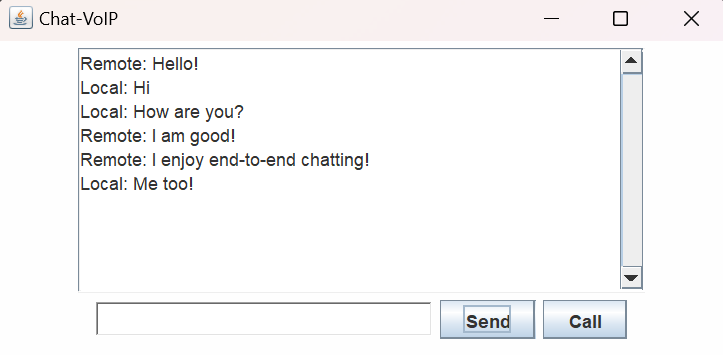
\includegraphics[width=1\linewidth]{assets/Chat.png}
    \caption{\textbf{Chat Interface}}
    \label{fig:chat-interface}
\end{figure}

\section{Chat Implementation}

The chat functionality is implemented using \textbf{UDP sockets}. A \textit{dedicated thread} is used to listen for incoming messages on \textbf{port 12345}. Outgoing messages are encrypted and sent via a \textit{separate thread} when the send button is pressed. Received messages are decrypted and displayed on the screen.

\subsection{Receiving Messages}
The following code snippet demonstrates the implementation of the listener thread for receiving messages:

\begin{lstlisting}[caption={\textbf{Receiving Messages}}, label={lst:receive-messages}]
// start a thread to listen for incoming messages
Thread receiveThread = new Thread(() -> {
    DatagramSocket socket = null;
    try {
        // listen to port 12345 for inbound text messages
        socket = new DatagramSocket(12345);
        byte[] buffer = new byte[1024];

        // continuously listen for incoming messages
        while(true) {
            DatagramPacket packet = new DatagramPacket(buffer, buffer.length);
            socket.receive(packet);
            String encryptedMessage = new String(packet.getData(), 0, packet.getLength());
            String message = app.decryptMessage(encryptedMessage);
            textArea.append("Remote: " + message + newline);
        }
    } catch(Exception ex) {
        ex.printStackTrace();
    } finally {
        if(socket != null && !socket.isClosed()) {
            socket.close();
        }
    }
});
receiveThread.start();
\end{lstlisting}

\subsection{Sending Messages}
When the send button is clicked, the following function is triggered, which encrypts and sends the message to the recipient.

\begin{lstlisting}[caption={\textbf{Sending Messages}}, label={lst:send-messages}]
private void handleSendButton() {
    try {
        // get user input
        String message = inputTextField.getText();
        String encryptedMessage = encryptMessage(message);
        byte[] buffer = encryptedMessage.getBytes();
        InetAddress receiverAddress = InetAddress.getByName("RECEIVER_IP"); // replace with actual receiver IP
        int port = 12345; // message port
        DatagramPacket packet = new DatagramPacket(buffer, buffer.length, receiverAddress, port);
        
        DatagramSocket socket = new DatagramSocket();
        socket.send(packet);
        socket.close();
        
        textArea.append("Local: " + message + newline);
        inputTextField.setText("");
    } catch(Exception ex) {
        ex.printStackTrace();
    }
}
\end{lstlisting}

\vspace{0.5cm}
We can verify the text packet traffic on port 12345 with \textbf{Wireshark}, by using the correct filters.
\begin{figure}[H]
    \centering
    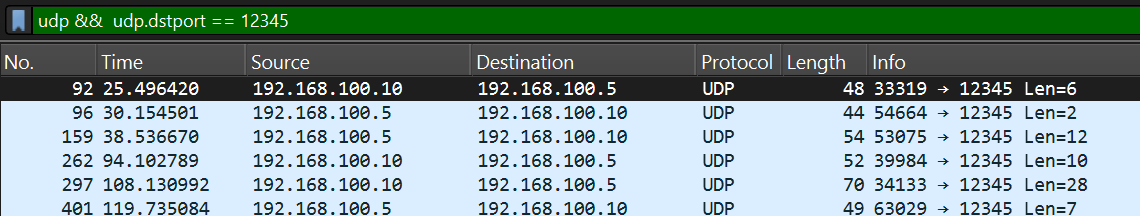
\includegraphics[width=1\linewidth]{assets/Chat Stream.png}
    \caption{\textbf{Packet Stream Analysis for Chat}}
    \label{fig:chat-stream}
\end{figure}

\vspace{0.5cm}
By clicking on an individual package we can further inspect it and reveal its \textbf{Network/Internet headers} and its \textbf{payload}.
\begin{figure}[H]
    \centering
    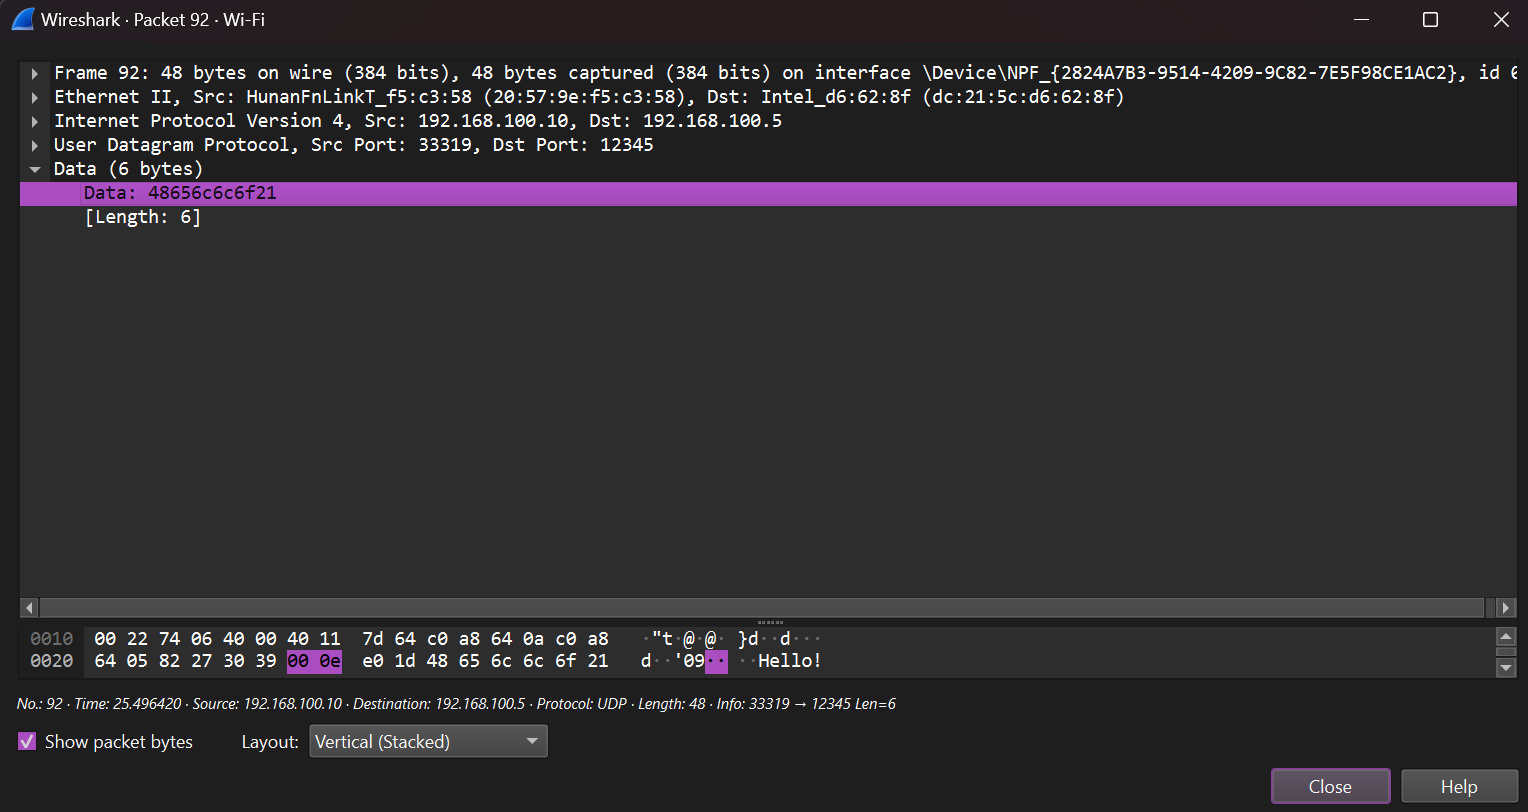
\includegraphics[width=1\linewidth]{assets/Text Package.png}
    \caption{\textbf{Individual Text Package}}
    \label{fig:enter-label}
\end{figure}

\section{VoIP Implementation}

The VoIP functionality allows \textit{real-time} voice communication. This is achieved using the \textbf{PCM audio format} with an 8000 Hz sample rate, 8-bit sample size, and a monophonic channel. Two threads manage audio transmission and reception using UDP on \textbf{port 12346}.

\subsection{Starting a Call}
The following function starts the call by creating \textit{separate threads} for audio sending and receiving:

\begin{lstlisting}[caption={\textbf{VoIP Call Implementation}}, label={lst:voip-call}]
private void handleCallButton() {
    callActive = true;

    Thread voiceThread = new Thread(() -> {
        final TargetDataLine[] microphone = new TargetDataLine[1];
        final SourceDataLine[] speaker = new SourceDataLine[1];
        try {
            AudioFormat format = new AudioFormat(8000, 8, 1, true, true); // PCM format
            DataLine.Info micInfo = new DataLine.Info(TargetDataLine.class, format);
            DataLine.Info speakerInfo = new DataLine.Info(SourceDataLine.class, format);

            microphone[0] = (TargetDataLine) AudioSystem.getLine(micInfo);
            speaker[0] = (SourceDataLine) AudioSystem.getLine(speakerInfo);

            microphone[0].open(format);
            speaker[0].open(format);

            microphone[0].start();
            speaker[0].start();

            sendSocket = new DatagramSocket();
            receiveSocket = new DatagramSocket(12346);

            InetAddress receiverAddress = InetAddress.getByName("RECEIVER_IP"); // Replace with actual receiver IP
            int port = 12346; // VoIP port
            byte[] buffer = new byte[1024];

            // Thread to capture and send audio
            Thread sendThread = new Thread(() -> {
                try {
                    while (callActive) {
                        int bytesRead = microphone[0].read(buffer, 0, buffer.length);
                        if (bytesRead > 0) {
                            DatagramPacket packet = new DatagramPacket(buffer, bytesRead, receiverAddress, port);
                            sendSocket.send(packet);
                        }
                    }
                } catch (Exception ex) {
                    ex.printStackTrace();
                } finally {
                    if (sendSocket != null && !sendSocket.isClosed()) {
                        sendSocket.close();
                    }
                }
            });
            sendThread.start();

            // Continuously receive and play audio
            while (callActive) {
                DatagramPacket packet = new DatagramPacket(buffer, buffer.length);
                receiveSocket.receive(packet);
                speaker[0].write(packet.getData(), 0, packet.getLength());
            }
        } catch (Exception ex) {
            ex.printStackTrace();
        } finally {
            if (microphone[0] != null) {
                microphone[0].close();
            }
            if (speaker[0] != null) {
                speaker[0].close();
            }
        }
    });
    voiceThread.start();
}
\end{lstlisting}

\vspace{0.5cm}
Once again, using \textbf{Wireshark} with the proper filters we can view the voice packet traffic on port 12346.

\begin{figure}[H]
    \centering
    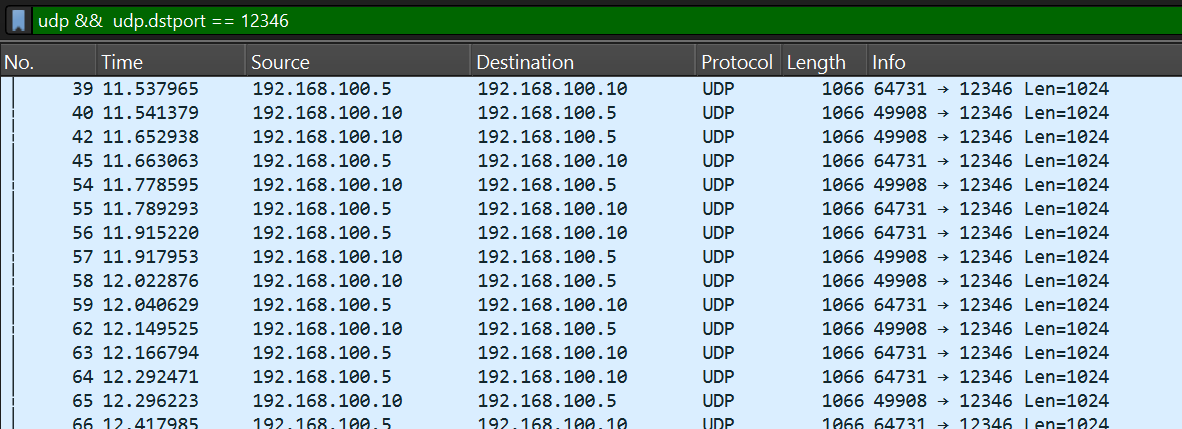
\includegraphics[width=1\linewidth]{assets/Call Stream.png}
    \caption{\textbf{Packet Stream Analysis for VoIP}}
    \label{fig:call-stream}
\end{figure}

By clicking on an individual package we can further inspect it and reveal its \textbf{Network/Internet headers} and its \textbf{payload}.
\begin{figure}[H]
    \centering
    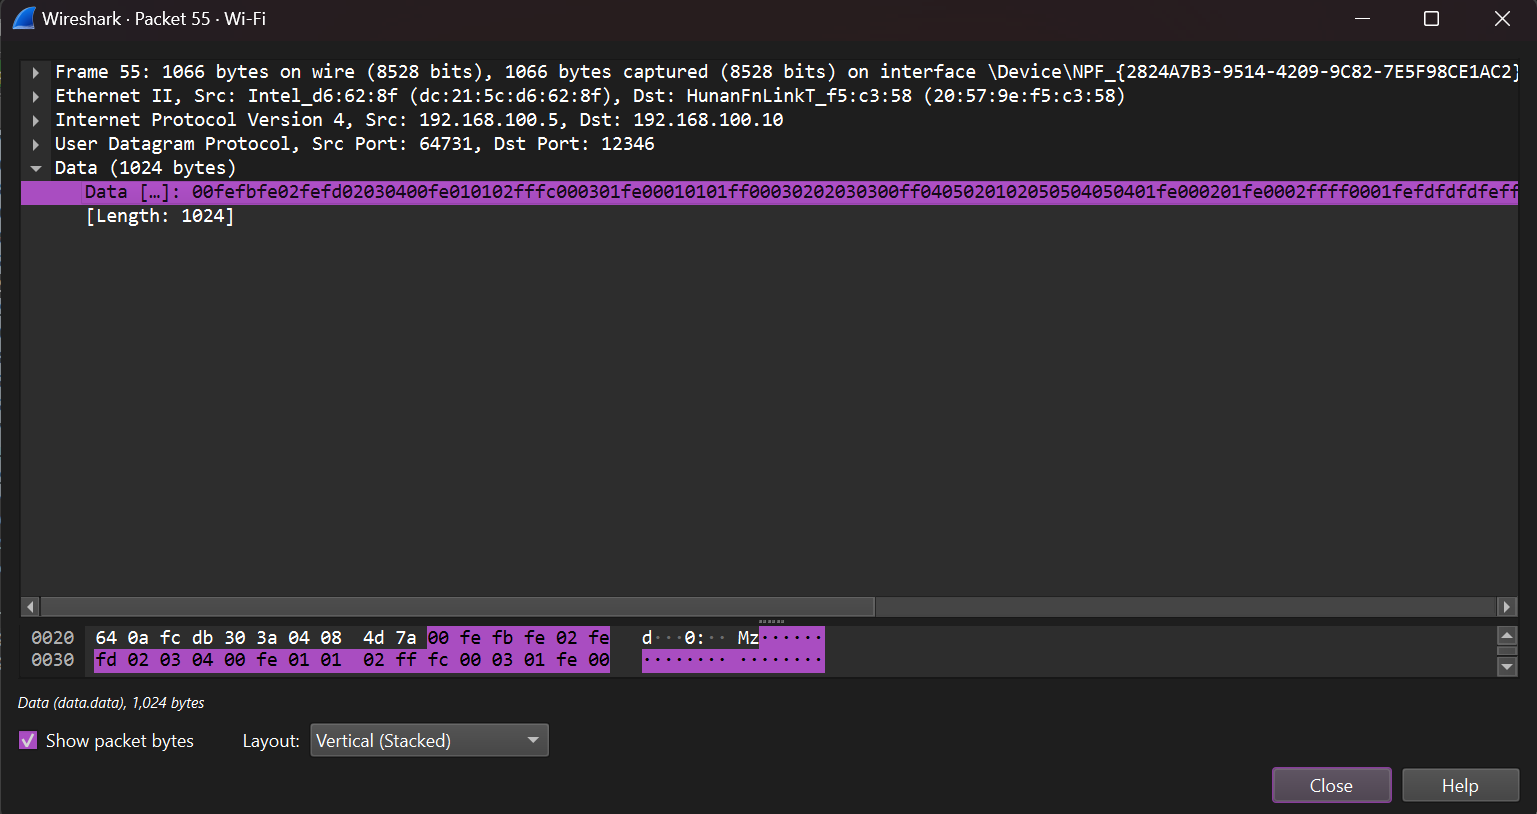
\includegraphics[width=1\linewidth]{assets/Voice Package.png}
    \caption{\textbf{Individual Voice Package}}
    \label{fig:enter-label}
\end{figure}

\section{Extras}

\subsection{Encryption}
If the packet is not encrypted, its contents are visible to anyone (as observed using \textbf{Wireshark}). To improve security, AES encryption was implemented for the chat messages, ensuring confidentiality. However, hardcoding the encryption key poses a potential vulnerability. To further secure the chat, the two users should securely exchange a shared key (using a method like the \textbf{Diffie-Hellman} method).

\begin{lstlisting}[caption={\textbf{Encryption and Decryption}}, label={lst:encryption}]
private String encryptMessage(String message) throws Exception {
    Cipher cipher = Cipher.getInstance("AES");
    cipher.init(Cipher.ENCRYPT_MODE, secretKey);
    byte[] encryptedBytes = cipher.doFinal(message.getBytes());
    return Base64.getEncoder().encodeToString(encryptedBytes);
}

private String decryptMessage(String encryptedMessage) throws Exception {
    Cipher cipher = Cipher.getInstance("AES");
    cipher.init(Cipher.DECRYPT_MODE, secretKey);
    byte[] decryptedBytes = cipher.doFinal(Base64.getDecoder().decode(encryptedMessage));
    return new String(decryptedBytes);
}
\end{lstlisting}

Here, we demonstrate the process of sending and receiving encrypted messaged using debug messages.
\begin{figure}[H]
    \centering
    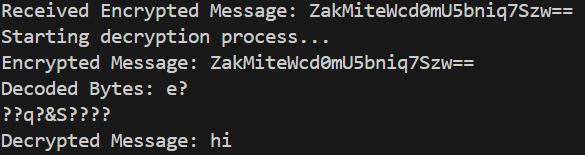
\includegraphics[width=1\linewidth]{assets/Terminal Encrypted.png}
    \caption{\textbf{Encrypted Chat}}
    \label{fig:enter-label}
\end{figure}

We see that now the packets appear encrypted in \textbf{Wireshark} as well.
\begin{figure}[H]
    \centering
    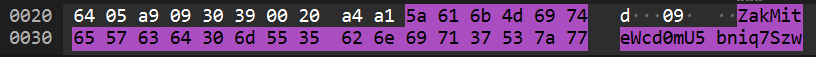
\includegraphics[width=1\linewidth]{assets/Encrypted Message.png}
    \caption{\textbf{Encrypted Packet}}
    \label{fig:encrypted-message}
\end{figure}

\section{Tools}
\begin{itemize}
    \item \textbf{Programming Language:} Java
    \item \textbf{IDE:} VSCode
    \item \textbf{Build Tool:} Maven
    \item \textbf{Version Control:} Git
    \item \textbf{Packet Analysis:} Wireshark
\end{itemize}

\end{document}